\documentclass[../TDO4.tex]{subfiles}%

\begin{document}
\section[s]"1"{Élargissement d'un faisceau laser}
\QR{%
	Un laser est un faisceau lumineux cylindrique dont le diamètre est de l'ordre
	du millimètre. On veut élargir ce faisceau jusqu'à lui donner un diamètre de
	quelque centimètres, en utilisant une lentille divergente et une lentille
	convergente. \textbf{Donner la relation entre les deux distances
		focales pour réaliser cet élargissement}. On prendra $d = \SI{2}{mm}$ le
	diamètre du faisceau entrant, et $D = \SI{3}{cm}$ celui du faisceau sortant.
}{%
	\ifstudent{%
		~
		\smallbreak
		\noindent
		\vspace{-15pt}
	}%
	\begin{minipage}{0.65\linewidth}
		On peut associer deux lentilles, la première divergente de très courte
		focale $f'_1$ ($< 0$) et la seconde convergente de grande focale $f'_2$, à
		condition de faire coïncider le foyer image $F'_1$ de la première avec le
		foyer objet $F_2$ de la seconde. Si $D$ est le diamètre du faisceau final et
		$d$ celui du faisceau initial, alors en utilisant le théorème de Thalès
		$D/f'_2 = -d/f'_1$~; pour $d = \SI{2}{mm}$ et $D = \SI{3}{cm}$, il nous faut
		\[
			f'_2 = -15 f'_1
		\]
	\end{minipage}
	\hfill
	\begin{minipage}{0.30\linewidth}
		\begin{center}
			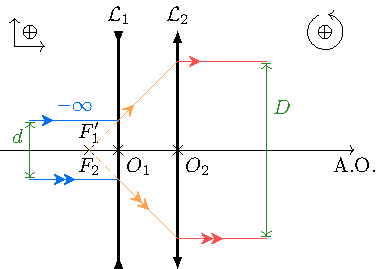
\includegraphics[width=\linewidth]{laser_elarg.pdf}
		\end{center}
	\end{minipage}
}%

\end{document}
